% !TEX program = xelatex
% ---------------------------------------------------------------------------
% PageRank 算法小引 —— 用一张五个点的小图走完整个排序计算
% 编译：xelatex PageRank算法小引.tex （跑两遍以刷新目录/引用）
% ---------------------------------------------------------------------------
\documentclass[UTF8,11pt,fontset=macnew]{ctexart}

\usepackage[a4paper,margin=2.4cm]{geometry}
\usepackage{amsmath,amssymb}
\usepackage{booktabs}
\usepackage{array}
\usepackage{enumitem}
\usepackage{xcolor}
\usepackage{tikz}
\usetikzlibrary{arrows.meta,positioning,calc}
\usepackage[most]{tcolorbox}
\usepackage{hyperref}

\definecolor{caramel}{HTML}{A9713C}
\definecolor{rosec}{HTML}{D8678F}
\definecolor{paper}{HTML}{FBF4EA}
\definecolor{inkc}{HTML}{3B2E24}

\hypersetup{colorlinks=true,linkcolor=caramel,urlcolor=rosec,
            pdftitle={PageRank 算法小引},pdfauthor={米露}}

\linespread{1.13}
\setlength{\parskip}{0.35em}
\setlist{itemsep=0.15em,topsep=0.3em}

\newtcolorbox{keybox}[1][小结]{breakable,enhanced,colback=paper,colframe=caramel,
  boxrule=0.7pt,arc=1.5mm,left=3mm,right=3mm,top=2mm,bottom=2mm,
  title={\bfseries #1},coltitle=white,colbacktitle=caramel,fonttitle=\bfseries}

\newtcolorbox{warnbox}[1][注意]{breakable,enhanced,colback=rosec!6,colframe=rosec,
  boxrule=0.7pt,arc=1.5mm,left=3mm,right=3mm,top=2mm,bottom=2mm,
  title={\bfseries #1},coltitle=white,colbacktitle=rosec,fonttitle=\bfseries}

\newcommand{\xv}{\mathbf{x}}
\newcommand{\one}{\mathbf{1}}

\title{\bfseries PageRank 算法小引\\[0.35em]
  \large 用一张五个点的小图，走完一遍排序计算}
\author{米露的读书笔记}
\date{2026 年 10 月}

\begin{document}
\maketitle
\pagestyle{plain}
\thispagestyle{empty}

\begin{keybox}[这篇文章想做的事]
PageRank 的公式写出来只有一行，但第一次看的人常常有三个疑问：
那个阻尼因子 $\alpha$ 到底是干什么的？悬挂点为什么要单独处理？
以及——这套东西真的能用手算出来吗？

这篇文章只用一张\textbf{五个点}的有向图做例子。这张图小到可以用纸笔算完，
但它同时包含了普通点、悬挂点、环、自环（封闭子集）这几种情况，
也就是 PageRank 需要打的\textbf{全部}补丁。
读完之后，你应该能自己动手把这张图的排名算出来。
（本文由大肥鱼写作）
\end{keybox}

\section{引子：怎么给网页排队}

搜索引擎要回答的第一个问题不是「哪个网页包含关键词」——那是检索的事——
而是「在命中关键词的一堆网页里，哪个更值得排在前面」。

PageRank 的想法很朴素，来自两条几乎人人都有的直觉：

\begin{enumerate}
  \item \textbf{被很多网页链接的网页，多半比较重要。}
  \item \textbf{来自重要网页的链接，比来自无关网页的链接更有分量。}
        而且一个网页链出去的链接越多，每条链接分到的分量就越被稀释——
        一个页面上堆了两百个友情链接，其中一条就不值钱了。
\end{enumerate}

把这两条合起来，就是「\textbf{随机冲浪者}」模型：想象一个无聊的人，
他不停地随机点击当前页面上的链接。一个网页越重要，
他长期来看停留在那个网页上的时间比例就越高。

于是我们给每个网页 $i$ 记一个分数 $x_i$，含义是
\[
x_i \;=\; \text{随机冲浪者长期停留在网页 } i \text{ 的时间比例},
\]
并要求
\[
x_i \ge 0, \qquad \sum_i x_i = 1 .
\]
所有网页的分数排成一个列向量 $\xv=(x_A,x_B,\dots)^\top$，它就是我们要的东西。
注意这是一个\textbf{概率分布}——这正是后面能借用线性代数的原因。

\section{例子：一张五个点的小图}

\begin{figure}[htbp]
\centering
\begin{tikzpicture}[
  vtx/.style={circle,draw=caramel,thick,fill=white,inner sep=1.4pt,
              minimum size=7.5mm,font=\sffamily\bfseries},
  edge/.style={-{Stealth[length=2.4mm]},thick,draw=caramel},
  special/.style={-{Stealth[length=2.4mm]},thick,draw=rosec},
  lbl/.style={font=\scriptsize,text=inkc,align=center}
]
\node[vtx] (A) at (0,0.5)      {A};
\node[vtx] (B) at (2.5,1.25)   {B};
\node[vtx] (C) at (1.1,-1.5)   {C};
\node[vtx] (D) at (3.7,-1.4)   {D};
\node[vtx,draw=rosec] (E) at (5.7,0.5) {E};

\draw[edge] (A) -- (B);
\draw[edge] (A) -- (C);
\draw[edge] (B) -- (C);
\draw[edge] (B) -- (D);
\draw[edge] (C) to[bend left=40] (A);
\draw[special] (E) to[loop above,looseness=5.5] (E);

\node[lbl,below=1.2mm of D] {出度 $0$};
\node[lbl,below=1.2mm of E,text=rosec] {自环};
\end{tikzpicture}
\caption{五个点的链接图。箭头表示「谁链接到谁」。}
\label{fig:main}
\end{figure}

每个点的出链（它链出去的网页）和出度（出链的条数）如下：

\begin{center}
\begin{tabular}{c c c}
\toprule
网页 & 它链接到 & 出度 \\
\midrule
A & B, C            & 2 \\
B & C, D            & 2 \\
C & A               & 1 \\
D & （谁也不链）      & 0 \\
E & E（自己）        & 1 \\
\bottomrule
\end{tabular}
\end{center}

这张图小，但把该踩的坑都踩了一遍：

\begin{itemize}
  \item \textbf{出度有 2、有 1、有 0}。出度 1 和 2 是常规情况
        （分数按出链均分）；出度 0 的点叫\textbf{悬挂点}（dangling node），
        它是个麻烦，第 \ref{sec:trouble} 节会看到。
  \item \textbf{A$\to$B$\to$C$\to$A 构成一个环}。纯按链接走的话，
        冲浪者会被这个环「卡住」，一圈一圈地转。
  \item \textbf{E 只有一条指向自己的边，而且没有任何别的网页链接到 E}。
        这样的 E 是一个\textbf{封闭子集}：一旦冲浪者走进去，就再也出不来。
        这是最阴险的一种情况，因为它会让别的网页全都拿不到分。
\end{itemize}

\section{线性代数准备：把图变成矩阵}
\label{sec:matrix}

\subsection{三件要用的东西}

只用三个概念，都是线性代数课本里的。

\begin{keybox}[三个概念]
\textbf{概率向量}：各分量非负、加起来等于 $1$ 的向量。
比如 $\xv=(0.2,0.2,0.2,0.2,0.2)^\top$（五点均分）就是一个概率向量。

\textbf{列随机矩阵}：所有元素非负，且\textbf{每一列的和都是 $1$} 的方阵 $M$。
它的用途是把一个概率向量变成另一个概率向量，
即「走一步之后，概率质量怎么重新分配」。

\textbf{平稳分布}：如果概率向量 $\boldsymbol{\pi}$ 满足
\[
\boldsymbol{\pi} = M\boldsymbol{\pi},
\]
就称它是 $M$ 的平稳分布。用线性代数的话说，
$\boldsymbol{\pi}$ 就是 $M$ 的、属于特征值 $\lambda = 1$ 的特征向量。
\end{keybox}

PageRank 的全部数学内容可以概括成一句话：
\textbf{构造一个合适的列随机矩阵，再求出它的平稳分布。}

\subsection{为什么求的是平稳分布}

迭代 $k$ 步就是
\[
\xv^{(k+1)} = M\,\xv^{(k)} .
\]
如果 $\xv^{(k)}$ 收敛到某个 $\xv^*$，那么两边取极限就得到
$\xv^* = M\xv^*$——极限必然是一个平稳分布。
所以「求平稳分布」和「反复迭代直到不动」是同一件事的两种说法。
后者叫\textbf{幂迭代}（power iteration），是我们实际动手算时用的方法。

至于为什么这样的平稳分布存在、而且唯一：当 $M$ 的每个元素都严格大于 $0$
时，Perron--Frobenius 定理保证模最大的特征值是 $1$ 且是单重的，
对应的特征向量可以取成每个分量都为正的向量，再归一化就是唯一的平稳分布。
我们后面构造的矩阵恰好就是这种「正矩阵」。

\subsection{先写出「裸」的转移矩阵}

先把链接关系原样写成矩阵，不做任何修补。
规则是：若网页 $j$ 链接到网页 $i$，则让 $i$ 分到 $j$ 的
$\dfrac{1}{\text{出度}(j)}$。记这个矩阵为 $S$：
\[
S_{ij} =
\begin{cases}
\dfrac{1}{\text{出度}(j)}, & j \text{ 链接到 } i,\\[2mm]
0, & \text{否则}.
\end{cases}
\]

这里下标的意思要记牢：\textbf{列是「从哪来」，行是「到哪去」}。
$\xv^{(k+1)} = S\xv^{(k)}$ 恰好表示「走一步之后的质量分布」。

按这张图写出 $S$（第一列是行标签，第一行是列标签）：

\[
S=\left(\begin{array}{c|ccccc}
   & A & B & C & D & E\\ \hline
A  & 0            & 0            & 1            & 0 & 0\\[1mm]
B  & \frac{1}{2}  & 0            & 0            & 0 & 0\\[1mm]
C  & \frac{1}{2}  & \frac{1}{2}  & 0            & 0 & 0\\[1mm]
D  & 0            & \frac{1}{2}  & 0            & 0 & 0\\[1mm]
E  & 0            & 0            & 0            & 0 & 1
\end{array}\right)
\]

逐列检查一下就明白了：第 A 列（来自 A）$=(0,\frac12,\frac12,0,0)^\top$，
因为 A 的两条出链分别指向 B 和 C，各得一半；
第 C 列是 $(1,0,0,0,0)^\top$，因为 C 只有一条出链指向 A，全部给它；
第 E 列是 $(0,0,0,0,1)^\top$，因为 E 只链接自己。

\begin{warnbox}[问题来了]
数一下各列的和：
\[
1,\quad 1,\quad 1,\quad \boxed{0},\quad 1 .
\]
\textbf{D 那一列全是零，列和为 $0$。}
$S$ 还不是列随机矩阵，于是 $S\xv$ 也不再是概率向量——
D 上本来带着的那份概率质量，走一步以后就\textbf{凭空消失了}。
\end{warnbox}

\section{三个麻烦，一个补丁}
\label{sec:trouble}

\subsection{麻烦一：悬挂点}

D 没有任何出链。随机冲浪者走到 D 就无路可走了。
数学上表现为 $S$ 的 D 列全为零，概率不守恒。

\textbf{补丁：}规定冲浪者到了 D 之后，直接在地址栏里随手敲一个网址。
「随手敲」最自然的模型是\textbf{均匀地}在所有页面里挑一个，即每个页面
各得 $1/n$（这里 $n=5$，即每页 $1/5$）。也就是把 D 看成
「指向所有页面（含它自己）各 $\frac15$ 条边」。

把 $S$ 的 D 列改成每项 $1/5$，记作 $\tilde S$：

\[
\tilde S=\left(\begin{array}{c|ccccc}
   & A & B & C & D & E\\ \hline
A  & 0            & 0            & 1            & \frac15 & 0\\[1mm]
B  & \frac{1}{2}  & 0            & 0            & \frac15 & 0\\[1mm]
C  & \frac{1}{2}  & \frac{1}{2}  & 0            & \frac15 & 0\\[1mm]
D  & 0            & \frac{1}{2}  & 0            & \frac15 & 0\\[1mm]
E  & 0            & 0            & 0            & \frac15 & 1
\end{array}\right)
\]

现在每列和都是 $1$，$\tilde S$ 是列随机矩阵了，概率不会再消失。
但光是这样还不够——看下去。

\subsection{麻烦二：环与周期性}

只保留 $\tilde S$（也就是暂时取 $\alpha=1$，见下节）会怎样？
先看一个比五个点更小的例子：两个网页互相链接，没有别的边。

\begin{center}
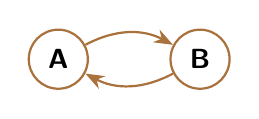
\begin{tikzpicture}[
  vtx/.style={circle,draw=caramel,thick,fill=white,inner sep=1.4pt,
              minimum size=7.5mm,font=\sffamily\bfseries},
  edge/.style={-{Stealth[length=2.4mm]},thick,draw=caramel}
]
\node[vtx] (A) at (0,0) {A};
\node[vtx] (B) at (1.8,0) {B};
\draw[edge] (A) to[bend left=28] (B);
\draw[edge] (B) to[bend left=28] (A);
\end{tikzpicture}
\end{center}

这时 $S=\begin{pmatrix}0&1\\1&0\end{pmatrix}$。
从 $\xv^{(0)}=(1,0)^\top$ 出发：
\[
(1,0)\;\to\;(0,1)\;\to\;(1,0)\;\to\;(0,1)\;\to\;\cdots
\]
质量在两个点之间来回弹，\textbf{永远不收敛}。
线性代数上，$S$ 的特征值是 $1$ 和 $-1$，那个 $-1$ 就是罪魁祸首——
主特征值不单重，平稳分布不唯一（$(1,0)$ 和 $(0,1)$ 都是），
幂迭代也就没有极限可言。这种结构叫\textbf{周期}的。

在我们的五个点里也有环（A$\to$B$\to$C$\to$A）。
这个环本身是 3 周期的，好在 A 还有一条边直达 C，多出一个 2 周期的
小环，两者一搅和，周期性被破坏了。所以五个点的例子里不会真的来回震荡，
但会撞上第三种麻烦——更糟的那种。

\subsection{麻烦三：封闭子集}

现在把 $\tilde S$ 直接拿去迭代（等价于取 $\alpha=1$），
从均匀的 $\xv^{(0)}=(0.2,0.2,0.2,0.2,0.2)^\top$ 出发，得到：

\begin{center}
\footnotesize
\begin{tabular}{c rrrrr}
\toprule
$k$ & $x_A^{(k)}$ & $x_B^{(k)}$ & $x_C^{(k)}$ & $x_D^{(k)}$ & $x_E^{(k)}$\\
\midrule
0  & 0.200000 & 0.200000 & 0.200000 & 0.200000 & 0.200000\\
1  & 0.240000 & 0.140000 & 0.240000 & 0.140000 & 0.240000\\
2  & 0.268000 & 0.148000 & 0.218000 & 0.098000 & 0.268000\\
3  & 0.237600 & 0.153600 & 0.227600 & 0.093600 & 0.287600\\
5  & 0.233424 & 0.142264 & 0.211024 & 0.087864 & 0.325424\\
10 & 0.205132 & 0.121763 & 0.184102 & 0.078515 & 0.410489\\
20 & 0.156634 & 0.092791 & 0.140458 & 0.059994 & 0.550122\\
40 & 0.091217 & 0.054038 & 0.081797 & 0.034938 & 0.738010\\
60 & 0.053121 & 0.031469 & 0.047635 & 0.020347 & 0.847429\\
\bottomrule
\end{tabular}
\end{center}

$E$ 的分数一路涨，其余四个点一路跌，最后全部趋于 $0$，$E$ 趋于 $1$。
排名彻底失去意义。

原因很清楚：E 只有一条指向自己的边，没有任何别的页面链接到 E，
所以一旦有质量流进 E（悬挂点 D 的「随手敲网址」正好会把质量送给 E），
它就再也不会离开。E 是个\textbf{吸收态}，别的点都在往这个无底洞里漏分。
这种情况下算法「收敛」了，但收敛到一个毫无用处的答案。

\begin{keybox}[小结：两种毛病的共同根源]
周期性让迭代震荡不收敛，封闭子集让迭代收敛到无用的答案。
它们的共同根源都是：\textbf{冲浪者只能沿着链接走}。
只要给他一个「随时可能不按链接、直接乱跳」的机会，
两个毛病就一起治好了。
\end{keybox}

\section{补丁：阻尼因子与 Google 矩阵}

假设冲浪者每走一步，都以概率 $\alpha$ 老老实实点一个链接，
以概率 $1-\alpha$ 不耐烦地在地址栏里重新敲一个网址（$n$ 个页面均匀挑一个）。
这个 $\alpha$ 就叫\textbf{阻尼因子}（damping factor）。

写成矩阵，就是著名的 Google 矩阵：
\[
\boxed{\;G \;=\; \alpha\,\tilde S \;+\; \frac{1-\alpha}{n}\,\one\one^\top\;}
\qquad
\one=(1,1,\dots,1)^\top,
\]
其中 $\one\one^\top$ 是全 $1$ 的 $n\times n$ 矩阵，
每一项都是 $\frac{1-\alpha}{n}$。

物理意义：第一项是「跟着链接走」的部分，
第二项是「随机乱跳」的部分，它给每个网页发一份完全相同的底分。

\subsection{为什么这一个补丁治好两个病}

\begin{itemize}
  \item \textbf{周期性没了。}随机乱跳意味着「从任何页面出发，
        下一步都可能到达任何页面（包括它自己）」。链不再有周期，
        特征值 $-1$ 之类的麻烦自动消失。
  \item \textbf{封闭子集失效了。}因为 $G$ 的每个元素都至少是
        $\frac{1-\alpha}{n}>0$，$G$ 是\textbf{正矩阵}。
        由 Perron--Frobenius 定理，特征值 $1$ 单重，
        平稳分布存在且唯一，「谁也无法独占所有分数」。
  \item \textbf{迭代一定收敛。}对任何两个概率向量 $\xv,\mathbf{y}$，
        \[
        G\xv-G\mathbf{y}=\alpha\tilde S(\xv-\mathbf{y}),
        \]
        （随机跳转项被减掉了），而 $\tilde S$ 保范数，
        所以 $\|G\xv-G\mathbf{y}\|_1\le \alpha\|\xv-\mathbf{y}\|_1$。
        每迭代一次，误差至少乘以 $\alpha$——这是一个压缩映射，
        极限存在且唯一。
\end{itemize}

顺手把上面那个两点的周期例子治一下。取 $\alpha=0.85$、$n=2$：
\[
G_2=0.85\begin{pmatrix}0&1\\1&0\end{pmatrix}
   +\frac{0.15}{2}\begin{pmatrix}1&1\\1&1\end{pmatrix}
   =\begin{pmatrix}0.075&0.925\\0.925&0.075\end{pmatrix},
\]
从 $(1,0)^\top$ 出发：
\[
(1,0)\to(0.075,\,0.925)\to(0.861,\,0.139)\to(0.193,\,0.807)\to\cdots\to(0.5,\,0.5).
\]
不再原地打转，而是在摆动中收敛到「各占一半」。摆动幅度每步缩小
$0.85$ 倍，所以看着慢，但它确实在收敛。

\subsection{本题的 Google 矩阵}

回到五个点的图。取经典的 $\alpha=0.85$，于是
\[
\alpha=0.85,\qquad \frac{1-\alpha}{n}=\frac{0.15}{5}=0.03 .
\]
把 $\tilde S$ 的每个元素乘 $0.85$ 再加 $0.03$：

\[
G=\left(\begin{array}{c|ccccc}
   & A & B & C & D & E\\ \hline
A  & 0.03  & 0.03  & 0.88  & 0.20 & 0.03\\[1mm]
B  & 0.455 & 0.03  & 0.03  & 0.20 & 0.03\\[1mm]
C  & 0.455 & 0.455 & 0.03  & 0.20 & 0.03\\[1mm]
D  & 0.03  & 0.455 & 0.03  & 0.20 & 0.03\\[1mm]
E  & 0.03  & 0.03  & 0.03  & 0.20 & 0.88
\end{array}\right)
\]
（每一列的和仍然是 $1$。可以自己挑一列验算一下。）

\begin{warnbox}[$\alpha$ 到底取多少]
$0.85$ 是 Brin 和 Page 在 1998 年那篇讲 Google 的论文里用的经验值，
后来的实现也大多在 $0.85$ 左右。
$\alpha$ 越大，结果越忠实于链接结构，但收敛越慢
（误差按 $\alpha^k$ 衰减），也越容易被 E 那种「自环陷阱」钻空子；
$\alpha$ 越小，越接近「所有网页平均分」，区分度越低。
它是一个权衡出来的数，不是从天上掉下来的。
\end{warnbox}

\section{手算整个排序过程}

\subsection{把矩阵乘法写成公式}

直接做 $5\times5$ 的矩阵乘法当然可以，但有一个更好用的写法。
把 $G=\alpha\tilde S+\frac{1-\alpha}{n}\one\one^\top$ 逐项展开，
再注意到迭代过程中 $\sum_j x_j^{(k)}$ 恒等于 $1$，就得到：

\[
x_i^{(k+1)}
=\underbrace{\frac{1-\alpha}{n}}_{\text{随机跳转的底分}}
\;+\;\alpha\Bigg(
\underbrace{\sum_{j\to i}\frac{x_j^{(k)}}{\text{出度}(j)}}_{\text{所有链接到 } i \text{ 的页面送给它的分}}
\;+\;\underbrace{\sum_{j\ \text{悬挂}}\frac{x_j^{(k)}}{n}}_{\text{悬挂点平摊出来的}}\Bigg)
\]

对照这张图，就是五个很短的式子（$\alpha=0.85$，$(1-\alpha)/n=0.03$）：

\begin{align*}
x_A^{(k+1)} &= 0.03 + 0.85\Big(x_C^{(k)} + \tfrac15 x_D^{(k)}\Big)\\[0.5mm]
x_B^{(k+1)} &= 0.03 + 0.85\Big(\tfrac12 x_A^{(k)} + \tfrac15 x_D^{(k)}\Big)\\[0.5mm]
x_C^{(k+1)} &= 0.03 + 0.85\Big(\tfrac12 x_A^{(k)} + \tfrac12 x_B^{(k)} + \tfrac15 x_D^{(k)}\Big)\\[0.5mm]
x_D^{(k+1)} &= 0.03 + 0.85\Big(\tfrac12 x_B^{(k)} + \tfrac15 x_D^{(k)}\Big)\\[0.5mm]
x_E^{(k+1)} &= 0.03 + 0.85\Big(\tfrac15 x_D^{(k)} + x_E^{(k)}\Big)
\end{align*}

把这五个式子读一遍，PageRank 就基本掌握了：
谁链到我，谁就把自己分数的一部分送给我；出链越多，每条送出的就越少；
悬挂点无处可送，干脆平摊给所有人；
最后每个人都白拿一份 $0.03$ 的底分。

\subsection{第一步，完整地算一遍}

从均匀分布出发：
\[
\xv^{(0)}=(0.2,\ 0.2,\ 0.2,\ 0.2,\ 0.2)^\top .
\]
代入上面的公式（每一步都把数字写出来）：

\begin{align*}
x_A^{(1)} &= 0.03 + 0.85\,(0.2 + 0.2\times 0.2)
           = 0.03 + 0.85\times 0.24 = \mathbf{0.234}\\
x_B^{(1)} &= 0.03 + 0.85\,(0.1 + 0.04)
           = 0.03 + 0.85\times 0.14 = \mathbf{0.149}\\
x_C^{(1)} &= 0.03 + 0.85\,(0.1 + 0.1 + 0.04)
           = 0.03 + 0.85\times 0.24 = \mathbf{0.234}\\
x_D^{(1)} &= 0.03 + 0.85\,(0.1 + 0.04)
           = 0.03 + 0.85\times 0.14 = \mathbf{0.149}\\
x_E^{(1)} &= 0.03 + 0.85\,(0.04 + 0.2)
           = 0.03 + 0.85\times 0.24 = \mathbf{0.234}
\end{align*}

检查一下：$0.234+0.149+0.234+0.149+0.234=1$，概率没有丢。
注意这里每个式子里都出现了 $0.03$——那就是随机跳转发给每个人的底分，
它保证了没有人会被饿死。

\subsection{一直迭代下去}

同样的步骤重复下去（实际计算时当然交给计算机）：

\begin{center}
\footnotesize
\setlength{\tabcolsep}{7pt}
\begin{tabular}{c rrrrr}
\toprule
$k$ & $x_A^{(k)}$ & $x_B^{(k)}$ & $x_C^{(k)}$ & $x_D^{(k)}$ & $x_E^{(k)}$\\
\midrule
0  & 0.200000 & 0.200000 & 0.200000 & 0.200000 & 0.200000\\
1  & 0.234000 & 0.149000 & 0.234000 & 0.149000 & 0.234000\\
2  & 0.254230 & 0.154780 & 0.218105 & 0.118655 & 0.254230\\
3  & 0.235561 & 0.158219 & 0.224001 & 0.115953 & 0.266267\\
4  & 0.240112 & 0.149825 & 0.217068 & 0.116955 & 0.276039\\
5  & 0.234390 & 0.151930 & 0.215606 & 0.113558 & 0.284515\\
6  & 0.232570 & 0.148921 & 0.213491 & 0.113875 & 0.291143\\
7  & 0.230826 & 0.148201 & 0.211492 & 0.112650 & 0.296830\\
8  & 0.228919 & 0.147252 & 0.210237 & 0.112136 & 0.301456\\
10 & 0.226575 & 0.145780 & 0.207980 & 0.111180 & 0.308485\\
20 & 0.222088 & 0.143079 & 0.203929 & 0.109471 & 0.321432\\
60 & 0.221291 & 0.142607 & 0.203215 & 0.109166 & 0.323720\\
\bottomrule
\end{tabular}
\end{center}

开头几步晃得挺厉害（0.234 掉到 0.149 又回来），
但摆动幅度每步缩小 $0.85$ 倍，很快就稳住了。
到 $k=60$ 时已经和极限值相差不到 $2\times 10^{-6}$。
精确的极限值是
\[
\xv^*=\Big(\tfrac{212280}{959281},\ \tfrac{136800}{959281},\ \tfrac{194940}{959281},\
\tfrac{104721}{959281},\ \tfrac{310540}{959281}\Big)^{\!\top},
\]
五个分量之和恰好为 $1$。

\subsection{收敛判据与迭代次数}

实用的判据是：当相邻两次迭代的差 $\max_i|x_i^{(k+1)}-x_i^{(k)}|$
小于某个阈值（比如 $10^{-6}$）就停手。
由于误差按 $\alpha^k$ 衰减，所需迭代次数大约是
\[
k \;\approx\; \frac{\ln \varepsilon}{\ln \alpha},
\]
$\varepsilon$ 是要求的精度。$\alpha=0.85$ 时，
想精确到 $10^{-6}$ 大约需要 $60\sim 90$ 次迭代——
本例子中，迭代 61 次以后与极限的偏差就小于 $10^{-6}$ 了。
这也是 PageRank 在工程上可用的原因：每步只跟链接图有关，
迭代次数是个不大的常数，而且可以并行。

\section{结果解读}

收敛之后，把五个分数从大到小排：

\begin{center}
\begin{tabular}{c c l}
\toprule
名次 & 网页 & 分数 \\
\midrule
1 & E & 0.323722 \\
2 & A & 0.221291 \\
3 & C & 0.203215 \\
4 & B & 0.142607 \\
5 & D & 0.109166 \\
\bottomrule
\end{tabular}
\end{center}

有几个地方值得停下来想一想。

\textbf{E 排第一，但它其实是个「作弊」的页面。}
E 没有任何外部入链，只有一条指向自己的边，却拿了最高的分。
这是因为 $0.85$ 的质量每走一步都留在自己身上。
把 $E$ 那一行单独拿出来解，可以直接验证这个数：
\[
x_E = 0.03 + 0.85\Big(\frac{x_D}{5} + x_E\Big)
\;\Longrightarrow\;
x_E = \frac{0.03 + 0.17\,x_D}{0.15}
= \frac{0.03+0.17\times 0.109166}{0.15} = 0.323722 .
\]
自环就是 PageRank 的软肋：$\alpha$ 越接近 $1$，这种陷阱越占便宜。
现实里单靠自环刷排名的页面另有办法收拾，
但作为学习者，看到这个数应该记住：\textbf{PageRank 度量的是链接结构，
不是内容价值}。

\textbf{A 比 C 高，尽管 C 有两条入链，而 A 只有一条。}
这正是 PageRank 比「数入链条数」高明的地方：
C 的两条入链分别来自 A 和 B，各只给它一半的分（A 和 B 都链了两个页面）；
而 A 的那一条入链来自 C，C 只链了 A 一个页面，于是把全部的分都给了 A。
\textbf{「少而专注」的一票胜过「多而分散」的两票。}

\textbf{D 垫底。}
D 有一条入链（来自 B），但它自己不出链，
分数只能靠随机跳转的底分 $0.03$ 和 B 的半票，
还要被自己「悬挂平摊」分薄一点，于是落在最后。

\begin{keybox}[补一种没画进图里的情况]
如果某个页面\textbf{连一条入链都没有}（比如刚上线、还没人链接的新页面），
它的分数会退化成
\[
x = \frac{1-\alpha}{n} + \alpha\cdot\frac{x}{n}
\quad\Longrightarrow\quad
x = \frac{1-\alpha}{n-\alpha}
\;\stackrel{\alpha=0.85,\,n=5}{=}\; 0.0361 .
\]
也就是说，这样的页面不会得 $0$ 分，而是安安稳稳地拿一份「底薪」。
这正是阻尼因子 $\alpha<1$ 的好处：\textbf{没有任何页面会被彻底判死刑}。
\end{keybox}

\section{小结：PageRank 算法流程}

\begin{enumerate}
  \item 把网页和链接建成有向图。
  \item 写出转移矩阵 $\tilde S$：列 $j$ 表示「从 $j$ 出发」，
        质量按出链均分；\textbf{悬挂点（出度为 $0$）的列取 $1/n$ 均匀分布}。
  \item 加上阻尼：$G=\alpha\tilde S+\frac{1-\alpha}{n}\one\one^\top$，
        通常 $\alpha=0.85$。
  \item 从任意概率向量（一般取均匀分布）出发，做幂迭代
        $\xv^{(k+1)}=G\xv^{(k)}$，直到变化小于阈值。
  \item 按 $x_i$ 从大到小排，就是网页排名。
\end{enumerate}

\begin{itemize}
  \item \textbf{代价：}每迭代一次只需要处理一遍所有链接，
        复杂度为 $O(\text{边数})$；由于 $\alpha<1$，迭代次数是一个不大的常数。
  \item \textbf{实现细节：}实际系统\textbf{不会}真的构造 $G$——
        $G$ 是稠密矩阵，而真实网页图极其稀疏。
        做法是直接算 $\tilde S$ 的稀疏乘法，再加上常数项
        $\frac{1-\alpha}{n}$（这正是第 6 节公式里那个 $0.03$ 的来历）。
  \item \textbf{一个重要的性质：}排名只依赖链接结构，
        与用户查询的关键词无关。所以它可以在离线阶段算好，
        这也解释了当年 Google 为什么能把它做到全网规模。
\end{itemize}

\begin{keybox}[回头再看这张五个点的图]
现在可以回答开头的问题了。这张图之所以够用，是因为它同时包含了：
\textbf{出度 2 和 1 的普通点}（A、B、C）、
\textbf{悬挂点}（D，出度 $0$）、
\textbf{环}（A$\to$B$\to$C$\to$A，会造成周期与震荡）、
\textbf{自环与封闭子集}（E，会吞掉全部分数）。
PageRank 公式里每一个零件——均分、悬挂点修补、阻尼因子——
都能在这张图上找到它对应的、可以手算验证的位置。
\end{keybox}

\end{document}
